% !TeX root = ../main.tex
% Add the above to each chapter to make compiling the PDF easier in some editors.

\chapter{Related Work}\label{chapter:Related Work}
In this section i am going to inspect projects from third parties, who also did work related to recognizing traffic signs, explaining them and trying to point out which methods have been used and why.

\section{Computer Vision}
\subsection{OpenCV Based Road Sign Recognition on Zynq}
The paper by Matthew Russell and Scott Fischaber presents a system on chip approach with a Xilinx Zynq-7020 chip, for recognizing and classifying road signs. The methods for detection are color-based techniques paired with shape recognition, implemented with the OpenCV library. To finally classify the regions of interest, found in the first steps, template matching is used. The system's performance is around 0.2 frames per second \cite{zynq}. Subsequent paragraph is going to describe the methods used to extract certain regions, that might be important for the task of road sign detection, thus the green part of figure \ref{fig:zynq}. \newline
The first stage in the algorithm is
converting the image into the HSV color space, in order to remove background colors. HSV was chosen over HSI, because it is easier to implement in hardware, calculating  HSI requires more divisions and would therefore increase latency in hardware, resulting in an overall slowed down system. With the focus on red and blue traffic signs, red and blue pixels are being extracted and thresholded by the algorithm. Therafter Morphology  operations  are  applied  to  the  filtered 
image to recover some broken signs and to remove very small objects. After being converted to gray scale, the Canny Edge detection is being used, to determine every edge in given image, provided by OpenCV. 

\begin{figure}[H]
	\centering
	\minipage{0.6\textwidth}
	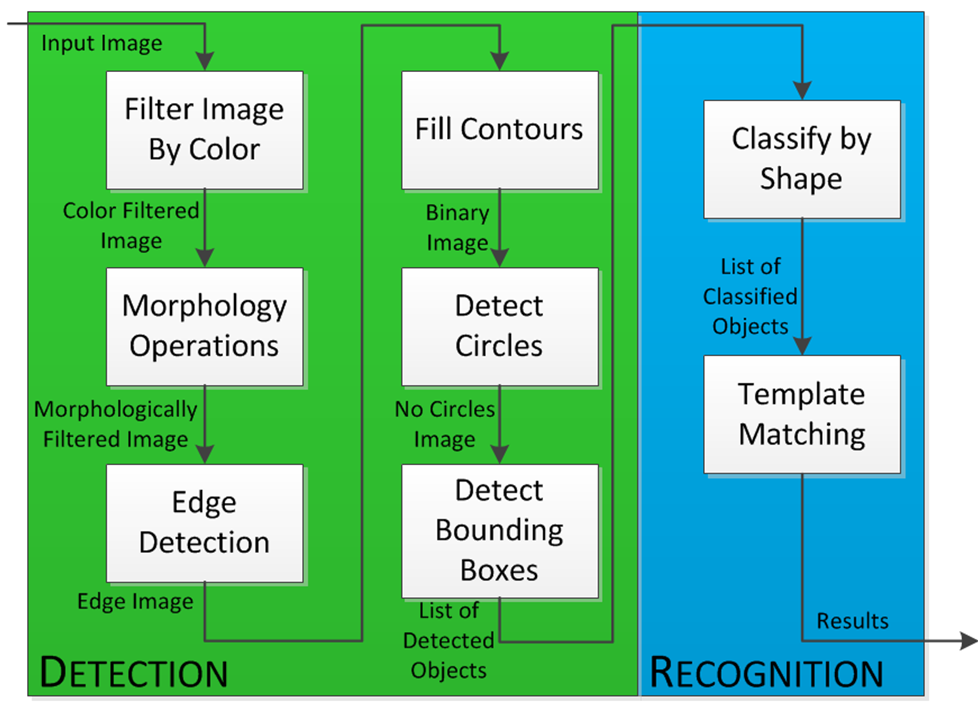
\includegraphics[width=\linewidth]{images/zynqconcept.png}
	\caption{Concept \cite{zynq}}\label{fig:zynq}
	\endminipage\hfill
\end{figure}

\section{Machine Learning}
\section{Deep Learning}